\providecommand{\main}{./report}
\documentclass[../main.tex]{subfiles}
\begin{document}


\section{Experiments}\label{section:experiments}
Accompanying the proposal of a new feature- ranking and selection methodology, an experiment is conducted. The aim of the experiment is to show an example of what is possible with both the pipeline, and the newly proposed evaluation methodology. In this way, \gls{ml} practitioners and authors of new methods are able to conduct experiments themselves with the same setup and configuration: therefore allowing comparison between the experiments.



\subsection{Experiment setup}
The experiment closely follows the outlines of Section~\ref{section:evaluation} and Section~\ref{section:pipeline}. The setup can be summarized like so:

\begin{itemize}
    \item The dataset at hand is split into a 80\% training- and 20\% testing dataset. Whereas the training set is reserved for fitting the feature ranker and validator, the testing set is reserved for scoring the validator.
    \item For each Feature Ranker and dataset, $B = 25$ bootstrap resampling iterations are run.
    \item In each bootstrap resampling iteration, $\min (p, 50)$ feature subsets are evaluated, with each including the $k$ best features.
    \item Validation estimators are evaluated with the R\textsuperscript{2} score in case of regression and with accuracy in the case of classification. The validation estimators used are \gls{knn} with $k=5$ and a \gls{dt} at default sklearn settings.
    \item In the aggregation process, in case several experimental runs are found with the same configuration, i.e., for one Feature Ranker executed on one dataset, only the `best' run is considered. The best run is considered to be the run with the highest average mean score over all features, considering all bootstraps. This aggregation step will be elaborated upon in Section~\ref{section:experiments-example}.
\end{itemize}

All experiments were run on a SLURM \gls{hpc} environment. Specifically, the University of Groningen has a `Peregrine' compute cluster, with machines of various types, of which the most common one is a 24 core machine powered by two Intel Xeon E5 2680v3 CPUs running at 2.5 GHz. Per node, 128 GB memory and 1 TB internal disk space is available, but 10 GB was requested per CPU instead. This accounts for a total of 100 GB memory for 10 CPU processes. The experiments took \todo{update amount of hours at end of thesis} 1700 hours to run on the above-mentioned machines.



\subsubsection{Experiment specification}
A line-up of feature rankers and datasets was constructed to conduct benchmarking on. See  Table~\ref{table:experiments-ranker-specification} for the Feature Ranking line-up, and Table~\ref{table:experiments-dataset-specification} for the datasets line-up.






%%% SYNCLF HARD %%
\subsection{Experimental results for the `Synclf hard' dataset}\label{section:experiments-example}
To best understand the format of the experimental results and the accompanying metrics, a look is taken at the results for one dataset. In this way, a better understanding of the charts is gained first. Also, because all results are freely accessible and available on an online dashboard\footnote{\href{https://wandb.ai/dunnkers/fseval}{https://wandb.ai/dunnkers/fseval}}\todo{'copy over to default dashboard'}, the reader is able to freely browse the results him- or herself, if he- or she desires so.

% `Synclf hard`
First of all, the considered dataset is the `Synclf hard' dataset. It is a synthetically generated dataset, created using the sklearn \texttt{make\_classification} function (Section~\ref{section:pipeline-components-datasets}). Its full configuration specification is defined in Listing~\ref{code:pipeline-synthetic-example}. The dataset is defined to have $n=10000$ samples and $p=50$ dimensions. After the \gls{cv} step was conducted, 8000 samples are left for training. The dataset has 4 relevant features and 3 target classes. That said, observations are first made on running one feature ranker on the dataset. For this, ReliefF \citep{kononenko_estimating_1994} is chosen.




\subsubsection{ReliefF on the `Synclf hard' dataset}
To start, a look is taken at a plot that explicitly plots \textbf{all bootstraps}. See Figure~\ref{fig:results-validation-dt-relieff}.

\begin{figure}[ht]
    \centering
    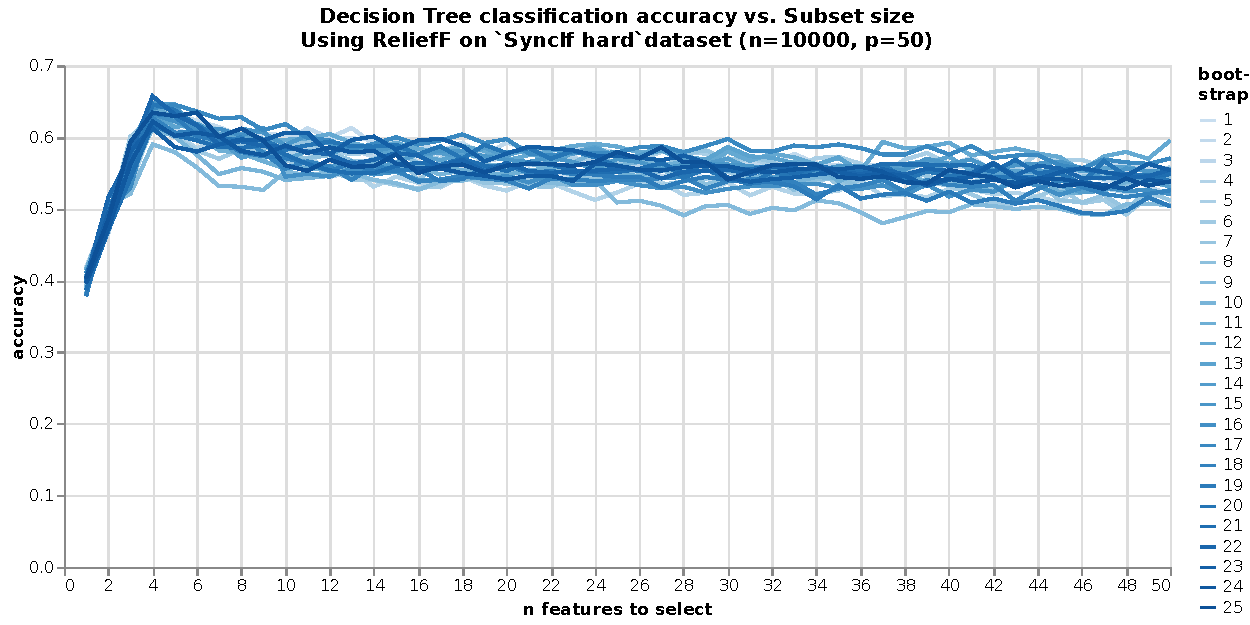
\includegraphics[width=\linewidth]{report/images/results-validation-dt-relieff.pdf}
    \caption{Validation performance for ReliefF on the `Synclf hard' dataset, for all 25 bootstraps.}
    \label{fig:results-validation-dt-relieff}
\end{figure}

As can be seen in Figure~\ref{fig:results-validation-dt-relieff}, the various bootstraps have had an effect on the validation performance per subset. Due to the random resampling with replacement taking place in the bootstrap phase, the feature ranker has to deal with permutations of the dataset each run. Indeed, this randomness is reflected in the validation performance.

One clear pattern is the fact that the validation performance first goes \textbf{up}, peaks at 4 features, and goes gradually down again. The fact that the peak happens at 4 features is clarified by the fact that the dataset had 4 informative features defined, meaning that the feature ranker correctly ranked the four informative features in its top-4 in most bootstraps. An intuition for the performance degradation is the fact that adding noisy dimensions can actually cause the estimator performance to degrade.

Next, a better look is taken at the estimated \textbf{feature importances}. Since the validation performance suggests that the ranker correctly identifies the importance of the informative feature, it is expected that this is reflected in the feature importance estimates. Indeed, this is the case. See Figure~\ref{fig:results-importances-relieff}.\todo{negative values? needs proper normalization}
\begin{figure}[ht]
    \centering
    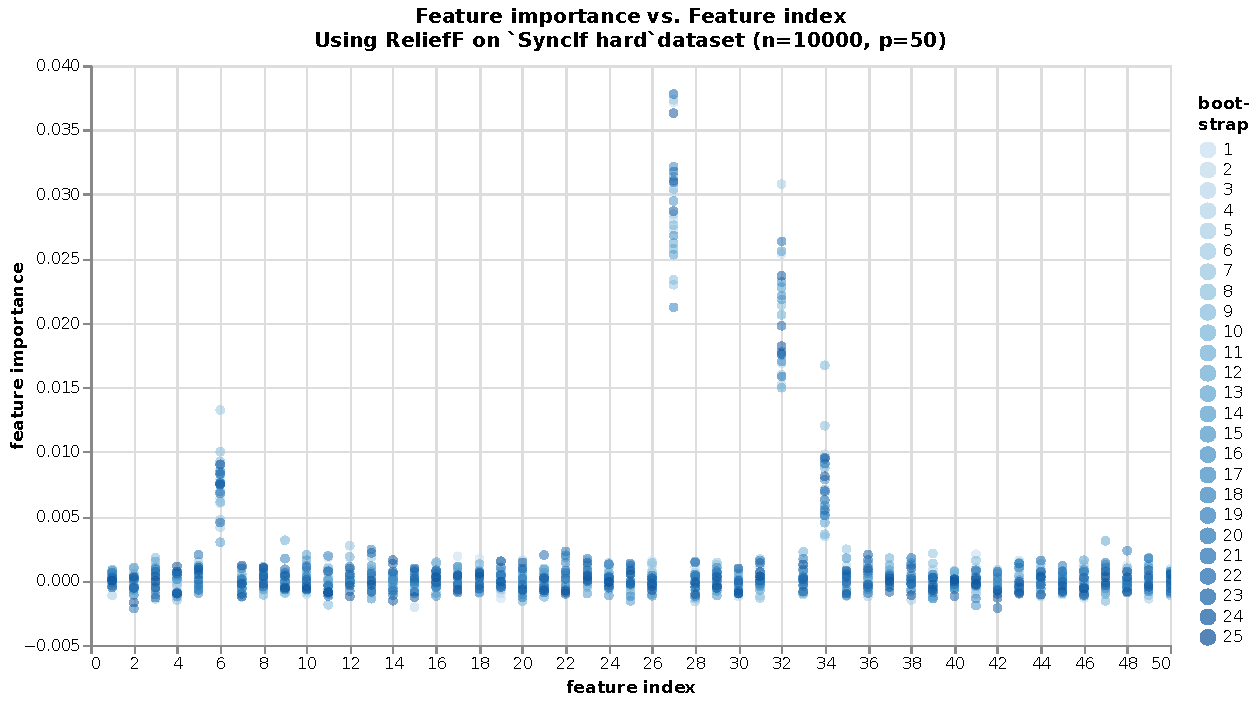
\includegraphics[width=\linewidth]{report/images/results-importances-relieff.pdf}
    \caption{Estimated feature importances for ReliefF on `Synclf hard'.}
    \label{fig:results-importances-relieff}
\end{figure}

It can be seen in Figure~\ref{fig:results-importances-relieff} that four features were assigned a larger importance than the others.  Indeed, these are the ground-truth relevant features, as is known \gls{apriori} because the dataset was synthetically generated. \todo{really, what are the ground-truth relevant features in this case? gotta check.}




\subsubsection{Multiple rankers on the `Synclf hard' dataset}
Next, multiple rankers are considered. Again, the dataset at hand is the `Synclf hard' dataset. The validation performance of all rankers can now be compared in a single plot, see Figure~\ref{fig:results-validation-dt-various-rankers}.

\begin{figure}[ht]
    \centering
    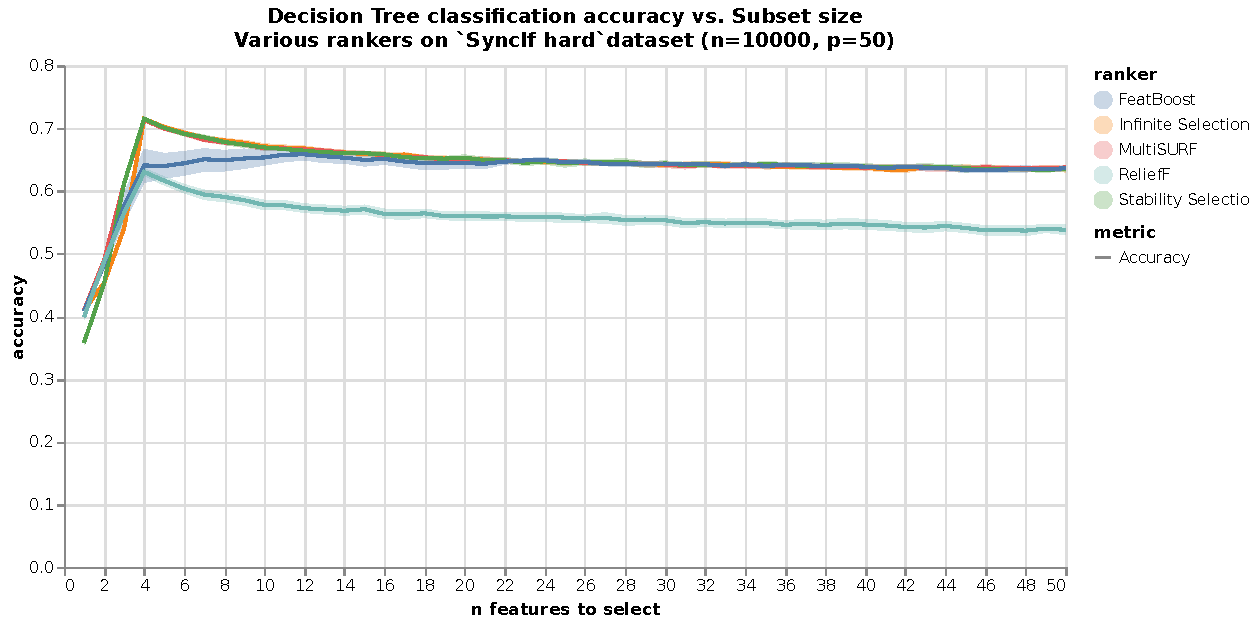
\includegraphics[width=\linewidth]{report/images/results-validation-dt-various-rankers.pdf}
    \caption{Validation performance of several rankers on the `Synclf hard' dataset.}
    \label{fig:results-validation-dt-various-rankers}
\end{figure}

Indeed, the various rankers show similar behavior in the validation performance. The performance of 


\begin{figure}[ht]
    \centering
    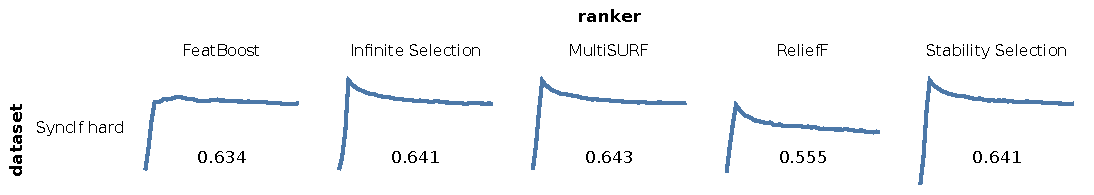
\includegraphics[width=\linewidth]{report/images/results-validation-with-mean-score.pdf}
    \caption{.}
    \label{fig:results-validation-with-mean-score}
\end{figure}

\begin{figure}[ht]
    \centering
    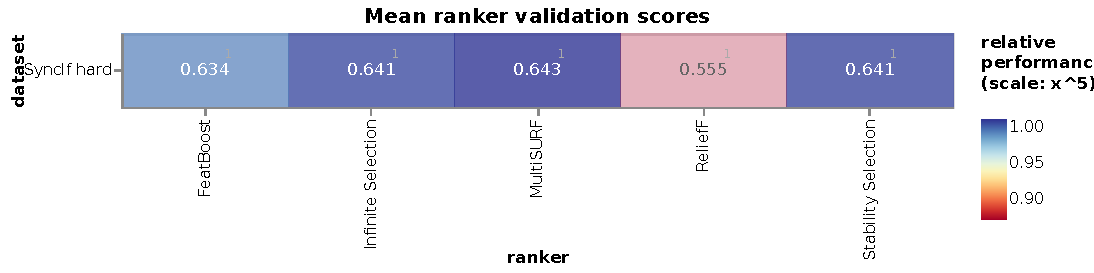
\includegraphics[width=\linewidth]{report/images/results-validation-with-mean-score-tabular.pdf}
    \caption{.}
    \label{fig:results-validation-with-mean-score-tabular}
\end{figure}


\begin{figure}[ht]
     \centering
     \begin{subfigure}[b]{0.48\textwidth}
        \centering
        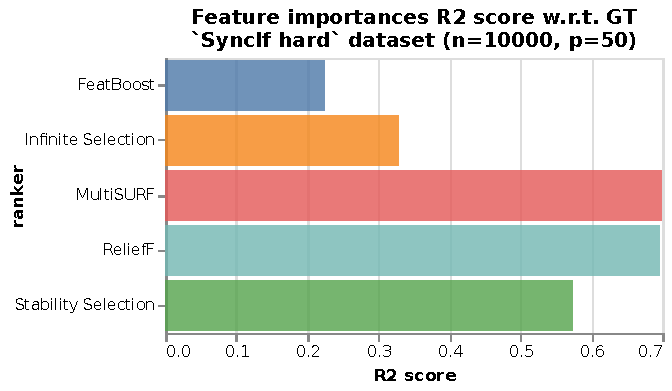
\includegraphics[width=\linewidth]{report/images/results-r2-score-various-rankers.pdf}
        \caption{.}
        \label{fig:results-r2-score-various-rankers}
     \end{subfigure}
     \hfill
     \begin{subfigure}[b]{0.48\textwidth}
        \centering
        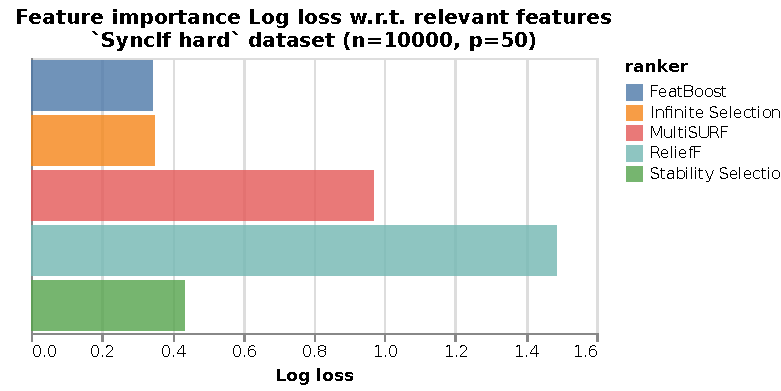
\includegraphics[width=\linewidth]{report/images/results-log-loss-various-rankers.pdf}
        \caption{.}
        \label{fig:results-log-loss-various-rankers}
     \end{subfigure}
     
    \caption{.}
    \label{fig:results-ground-truth-various-rankers}
\end{figure}








%%% ALL RESULTS %%
\subsection{Experimental result tables}
\subsubsection{Validation performance}
\subsubsection{Stability}
\subsubsection{Time complexity}




\biblio
\end{document}
